\documentclass[aspectratio = 169, 12pt]{beamer}
%
% Choose how your presentation looks.
%
% For more themes, color themes and font themes, see:
% http://deic.uab.es/~iblanes/beamer_gallery/index_by_theme.html
%
\mode<presentation>
{
  \usetheme{default}      % or try Darmstadt, Madrid, Warsaw, ...
  \usecolortheme{default} % or try albatross, beaver, crane, ...
  \usefonttheme{default}  % or try serif, structurebold, ...
  \setbeamertemplate{navigation symbols}{}
  \setbeamertemplate{caption}[numbered]
} 

%Header color
\setbeamercolor{title}{fg=brown}
\setbeamercolor{frametitle}{fg = purple}

%Page numbers
\addtobeamertemplate{navigation symbols}{}{%
    \usebeamerfont{footline}%
    \usebeamercolor[fg]{footline}%
    \hspace{1em}%
    \insertframenumber/\inserttotalframenumber
}

%Figures per chapter
\usepackage{chngcntr}
\counterwithin*{figure}{lecture}


%packages
\usepackage[english]{babel}
\usepackage[utf8]{inputenc}
\usepackage[T1]{fontenc}
\usepackage{graphicx}
\usepackage[default]{lato} %font
\usepackage{hyperref}
\hypersetup{
    colorlinks = true,
    linkcolor = {blue},
    urlcolor = {magenta}
}
\usepackage{verbatim}

%Table of contents markup
\usepackage{etoolbox}
\makeatletter
\patchcmd{\beamer@sectionintoc}
  {\vfill}
  {\vskip\itemsep}
  {}
  {}
\makeatother  
 

\AtBeginSection[]
{
\begin{frame}
\frametitle{Outline}
\tableofcontents[currentsection]
\end{frame}
}


\title{Feedback session 1: Introduction}
\author[Bas Machielsen (RSM)]{Bas Machielsen}
\date{\today}
\institute[]{\normalsize Rotterdam School of Management \\
\texttt{\href{http://bas-m.netlify.app}{bas-m.netlify.app}} \hspace{5pt} \texttt{\href{http://github.com/basm92}{github.com/basm92}}}

\begin{document}
	\titlepage
	\clearpage
	\section{Welcome \& Introduction}
	
	\begin{frame}{Who am I?}
	    \begin{itemize}
	        \item Bas Machielsen
	        \item MSc degrees in Economics (RU) and Business Administration (UT)
	        \item PhD Student in Economic History at Utrecht University
	        \item Research: political connections, political economy, empirical economics
	        \item Teaching experience in Methodology, Programming, Corporate Finance
	        \item email: a.h.machielsen@uu.nl, machielsen@rsm.nl
	        \item Github: \url{www.github.com/basm92}
	    \end{itemize}
	\end{frame}
	
	\begin{frame}{Who are you?}
	    \begin{itemize}
	        \item Introduction Round
	        \item Personal Interests
	        \item Why do you find this topic interesting?
	        \item What do you think about when you hear the words political connections? What do you think might be causes and consequences?
	    \end{itemize}
	\end{frame}
	
	\begin{frame}{First Bachelor Thesis Feedback Session}
	    \begin{itemize}
		    \item Structure of the course
		    \begin{figure}
		        \centering
		        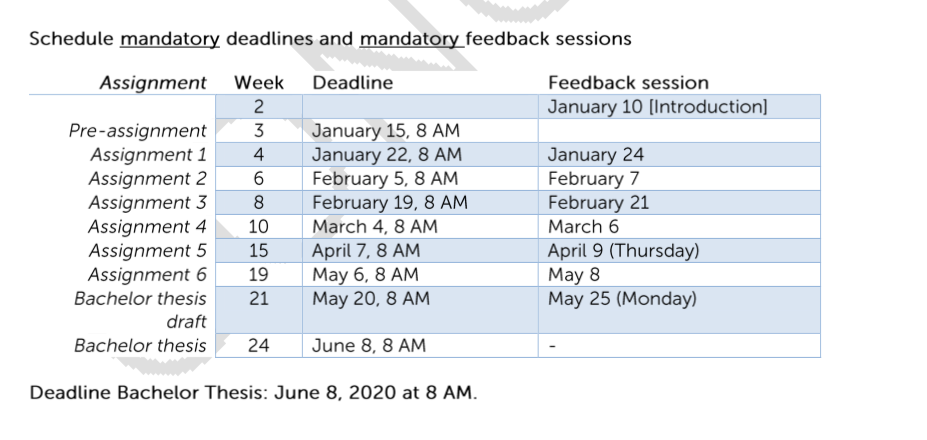
\includegraphics[width = 1.0\textwidth]{screen1.png}
		        \label{fig:my_label}
		    \end{figure}
		 \end{itemize}
	\end{frame}

	\begin{frame}{First Bachelor Thesis Feedback Session}
	    \begin{itemize}
	        \item All other sessions will feature \textit{group-based} feedback sessions, not collective sessions
	        \item In principle, dates and deadlines are fixed. 
	        \item Location: to be determined, I will let you know timely. I prefer 'social places', but we can also book rooms. 
	        \item Limited flexibility (regarding dates, not deadlines) is possible, contact me if you have any problems.
	        \item You should know all the dates well in advance. Time-slots will be allocated later.
	        \item I will communicate with you via Canvas announcements, but also via e-mail. 
	    \end{itemize}
	\end{frame}

\section{What to expect?}
    
	\begin{frame}{Prerequisite knowledge: Statistics}
		\begin{itemize}
		    \item You have all submitted a diagnostic test indicating your current ability to work with statistics
		    \item Mastering statistics is a very important component of doing empirical research, and without a knowledge of statistics, it is very difficult to understand any scientific literature 
		    \item If you have noticed that your score was unsatisfactory, you have to catch up
		\end{itemize}
	\end{frame}
	
	\begin{frame}{Catching up: How to do it?}
	    \begin{itemize}
	        \item Unfortunately, it is not my duty to help you catching up in statistics. 
	        \item I do, however, want to help you save effort by indicating the gravest bottlenecks (in my opinion), and some ways out. 
	        \item I want to focus on two things: Mastering statistical concepts, and getting and cleaning the data you need
	        \item I want to give you some resources you can use that have helped many students before you (including myself).
	    \end{itemize}
	\end{frame}
	
    \begin{frame}{Mastering statistical concepts}
        \begin{itemize}
            \item It makes sense that you can only understand a given approach to a question if you understand all the terms and concepts the author is using. 
            \item If you come across a sentence like "We used White standard errors to account for conditional heteroscedasticity", it will only be understandable what the authors did if:
                \begin{itemize}
                    \item you know what White standard errors are
                    \item you know what conditional heterscedasticity is. 
                \end{itemize}
            \item But before you can understand what White standard errors are, you have to know what standard errors are! 
            \item It often makes sense to 'decompose' a sentence and continually ask yourself what you don't understand
        \end{itemize}
    \end{frame}
    
    \begin{frame}{Statistical Concepts}
        \begin{itemize}
            \item Once you know this, you can aim your Google searches towards the building blocks of what you don't understand. 
            \item Aside from Google, here are some resources you can use
            \item First and foremost, your statistics textbook. 
            \item Secondly, \url{www.khanacademy.com} is an excellent website to catch up on statistics and, if necessary, high-school algebra
            \item Thirdly, on econometrics, there is the Youtube channel of \href{https://www.youtube.com/user/SpartacanUsuals}{\textbf{Ben Lambert}}, who provides econometrics courses at the undergraduate and graduate level. His explanations are very accessible. 
        \end{itemize}
    \end{frame}
    
    \begin{frame}{Statistical Concepts}
        \begin{itemize}
            \item In general, YouTube contains lots of good and free explanations of statistical concepts, tutorials to t-tests, ANOVA, regression analysis, etc., and the underlying mathematics
            \item There are also many paid and unpaid alternatives from academic sources. In particular, there are many courses teaching Statistics and Probability on \href{https://www.coursera.org/search?query=Statistics\%20and\%20probability}{Coursera}, \href{https://www.edx.org/course?search_query=Statistics}{EdX}, and \href{https://ocw.mit.edu/search/ocwsearch.htm?q=Statistics}{MIT OCW}. 
        \end{itemize}
    \end{frame}
    
    \begin{frame}{Getting, cleaning and analyzing data}
        \begin{itemize}
            \item This will become relevant as soon as you start analyzing your own data
            \item Many students find it difficult to go from raw, "downloaded" data to data that is ready for analysis
            \item Subsequently, many students have a hard time figuring out how to correctly analyse and interpret results
        \end{itemize}
    \end{frame}
    
    \begin{frame}{Getting, cleaning and analyzing data}
        \begin{itemize}
            \item Whether an tutorial or explanation is useful to you depends on the statistical program that you are using. 
            \item \href{https://www.coursera.org/learn/data-collection-analytics-project}{\textbf{This}} is a course that focuses on data collection and analysis and (sometimes) uses Stata.
            \item In addition, \href{https://www.youtube.com/user/statacorp/playlists}{\textbf{Stata's YouTube channel}} also features many useful tutorials, but also underlying theory!. 
            \item \href{https://www.youtube.com/watch?v=464NA2jPWlo}{\textbf{This video}} provides a good introduction on how to clean data in Stata.
            \item If you want to use R or Python, you can ask me for additional resources.
        \end{itemize}
        
    \end{frame}
	
	\begin{frame}{Quality and nature of feedback}
	    \begin{itemize}
		    \item Every time, I will carefully read the assignments sent in by you.
		    \item We have about half an hour per session to discuss, so I will focus on the content, rather than typo's.
		    \item You can expect that I come up with substantial and nontrivial feedback in language that you can understand.
		    \item Ask specific questions you want me to answer, and request specific feedback, to ensure that my feedback meets your desires.
		    \item You can always write in an email that you want me to focus on a particular aspect, and I will do so. 
		\end{itemize}
	\end{frame}
	
	\begin{frame}{What is important?}
	    \begin{itemize}
	        \item Theses will be graded based on quality of the analysis, learning, and understanding, not on whether a result is significant or not.
	        
	        \item Starting data collection early can help many problems and will also allow you to tackle your question more efficiently
	        
	        \item Deadline = Deadline: Time is the reason. I should have time to give you adequate feedback.
	        
	        \item Highlight the sections which you want me to look at and where my feedback is incorporated.
	    \end{itemize}
	    
	\end{frame}
	
\section{Political connections}
	\begin{frame}{The theme}
	    \begin{itemize}
	        \item Ties between businesses and politics have since long drawn the attention of the general public, but also of academics. 
	        \item Politicians are frequently accused of "cashing in" on their political career by joining the board of directors or board of supervisors of a prominent public company. 
	        \item Can you think of some reasons why politicians might join the board of firms? 
	        \item Can you think of some reasons why firms might chose to hire politicians, instead of other individuals?
	    \end{itemize}
	\end{frame}
	
	\begin{frame}{The theoretical framework}
	    \begin{itemize}
	        \item Political connections might be a specific case of a more general phenomenon called \textit{rent-seeking}.
	        \item Rent-seeking is defined as increasing one's own wealth without creating additional wealth. 
	        \item Can you think of any reasons why this might be so? 
	        \item Can you  think of situations in which political connections are costly to society? 
	        \item Can you identify factors on which the value of political connections to firms are dependent?
	    \end{itemize}
	\end{frame}
	
	\begin{frame}{Anecdotal Evidence}
	    \begin{figure}
	        \centering
	        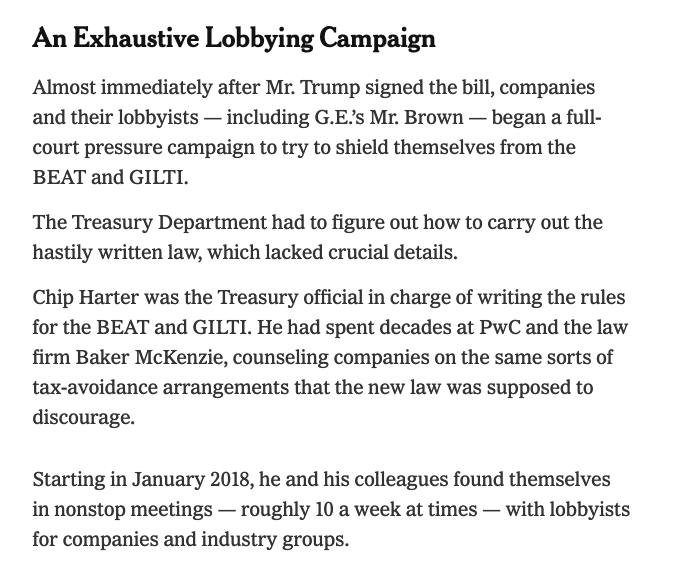
\includegraphics[scale = 0.33]{screen5.png}
	        \caption{Source: NY Times}
	        \label{fig:my_label}
	    \end{figure}
	\end{frame}
	
	\begin{frame}{From Anecdotal to Systematic Evidence}
	    \begin{itemize}
	        \item Source: \url{https://www.nytimes.com/2019/12/30/business/trump-tax-cuts-beat-gilti.html}
	        \item This article is about tax cuts in the US effectuated by the Trump administration. 
	        \item It is implied here that lobbying causes firms' tax burden to decrease. But is this benefit concentrated within politically connected firms?
	        \item Could political connections serve other purposes for firms other than lowering taxes?
	        \item Apart from anecdotal evidence of the kind reported in the above newspaper article, how would you go about testing these kind of theories?
	    \end{itemize}
	\end{frame}
	
	\begin{frame}{Empirical evidence}
	    \begin{itemize}
	        \item Fisman (2001) estimated the benefits of political connections by comparing politically connected firms to non-politically connected firms 
	        \item He estimated how the firm value responded to shocks in political connections in Indonesia, that were unanticipated by firms (arguably). 
	        \item The value of political connections could depend on a lot of things, including on who is the politician, and what the firm is like. 
	        \item Ferguson and Voth (2008) distinguish between politicians as executives and politicians on the supervisory board. What might be the reason they do so? 
	    \end{itemize}
	\end{frame}
	
	
	\begin{frame}{Differences between countries}
	    \begin{figure}
	        \centering
	        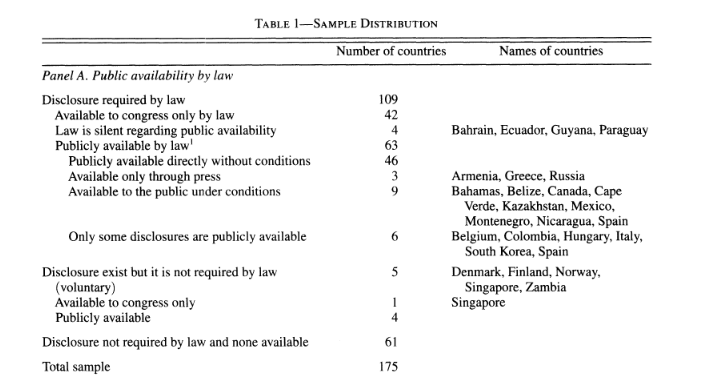
\includegraphics[width = 0.8 \textwidth]{screen7.png}
	        \label{fig:my_label}
	        \caption{\href{https://www.aeaweb.org/articles?id=10.1257/app.2.2.179}{Djankov et al., 2010, Disclosure by Politicians}}
	    \end{figure}
	\end{frame}
	
\section{Upcoming Assignments}
    \begin{frame}{Pre-Assignment}
        \begin{itemize}
            \item The pre-assignment focuses on teamwork and expectations, it will not be graded.
            \item More details: section 5, Course manual
        \end{itemize}
        \begin{figure}
            \centering
            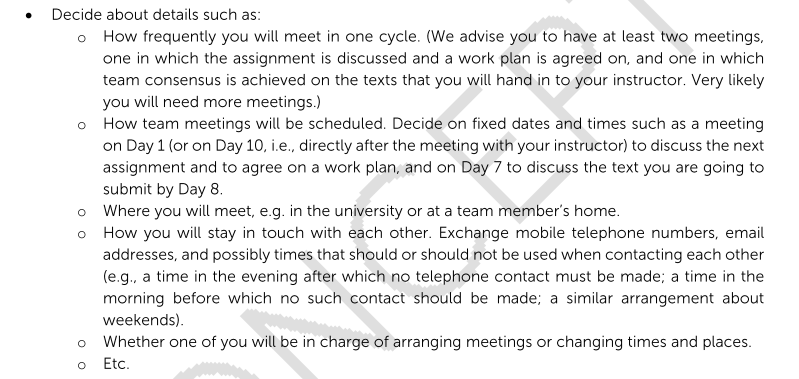
\includegraphics[width = 0.8 \textwidth]{screen6.png}
            \label{fig:my_label}
        \end{figure}
    \end{frame}

    \begin{frame}{Assignments: the way to go about this}
        \begin{itemize}
            \item Students read a chapter from the Course Book and watch the video
            \item Make an assignment
            \item Receive feedback from me
            \item Rework this into a thesis chapter
            \item It makes sense to show the 'cumulative' document to me
        \end{itemize}
    \end{frame}
    
    \begin{frame}{Questions}
        \begin{figure}
            \centering
            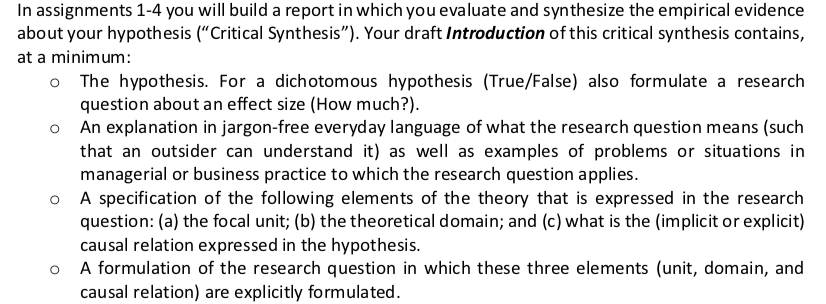
\includegraphics[width = 1.0\textwidth]{screen2.png}
            \label{fig:my_label}
        \end{figure}
    \end{frame}
    
    \begin{frame}{First article}
        \begin{itemize}
            \item I want you to use "Estimating the Value of Political Connections" by Raymond Fisman (AER, 2001) to be the first study you review. 
            \item This study was the first empirical study showing the existence of political connections, and spawned a new line of empirical research.
            \item The study also prompted questions as to why political connections are so beneficial, and what are the economic mechanisms that play a role. 
        \end{itemize}
    \end{frame}
    
    \begin{frame}{Additional studies}
        \begin{figure}
            \centering
            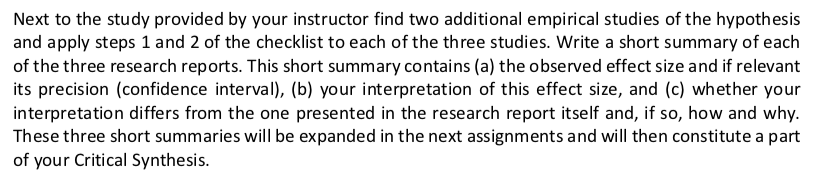
\includegraphics[width = 1.0 \textwidth]{screen3.png}
            \label{fig:my_label}
        \end{figure}
        \begin{itemize}
            \item You can pick either the 2nd study that is listed, or something else, but do search Google Scholar for other studies.
            \item You have to be able to explain the relevance of each study you include.
        \end{itemize}
    \end{frame}
    
    \begin{frame}{Coordination of times}
        \begin{itemize}
            \item Finally, I want to coordinate fixed times for each group.
            \item The locations can be variable. We can always go to a social corner.
            \item But if you prefer a less noisy environment, we can also arrange something else. 
        \end{itemize}
    
    \end{frame}
    
\section{More Resources}

    \begin{frame}{Course Theme Repository}
        \begin{itemize}
        \item I created a \href{https://github.com/Bachelor-Thesis-Political-Connections}{GitHub Repository}
        \item Content: walkthroughs (of various aspects that students found difficult in the past)
        \item For example: Programming and Data collection
        \item Also: research questions
        \item These lecture slides
        \end{itemize}
    \end{frame}
    
    \begin{frame}{Course Theme Repository [2]}
        \begin{itemize}
            \item You can also "copy" some of these scripts to your own system
            \item If you don't know how to do that, ask me!
            \item You can then change them and use them for your own purposes
            \item There are also some questions to get you started about thinking about your own RQ
            \item Examples based on these and other example RQs
            \item URL: \href{https://github.com/Bachelor-Thesis-Political-Connections/}{https://github.com/Bachelor-Thesis-Political-Connections/}
        \end{itemize}
    \end{frame}

\end{document}